\frame{
\frametitle{Diodi}
\begin{itemize}
\item Puolijohdediodi koostuu p- ja n-tyyppisen puolijohdepalasen rajapinnasta. n-tyyppisessä puolijohteessa on varauksenkuljettajina elektroneja ja p-tyyppisessä
aukkoja.
\item pn-liitoksessa virta voi kulkea vain toiseen suuntaan (pientä vuotovirtaa lukuunottamatta). Jos jännitteen kytkee toisin päin,
liitoksen ympärille muodostuu tyhjennysalue, ja varauksenkuljettajat eivät pääse liikkumaan.
\item Jos $U$ on positiivinen, sitä kutsutaan {\bf päästösuuntaiseksi} jännitteeksi, jos negatiivinen, {\bf estosuuntaiseksi}.
\end{itemize}

\begin{center}
\begin{picture}(100,40)(0,-10)
\rd{0,0}{}
\ri{10,0}{I}
\rcuu{0,10}{U}
\end{picture}
\end{center}
\[
I=I_{\rm S}\left(e^\frac{U}{nU_T}-1\right)\qquad U_T=\frac{{\rm k}T}{\rm q}
\]
\[
\rm q=1,602\cdot 10^{-19}\, {\rm As}\qquad {\rm k}=1,381
\cdot 10^{-23}\frac{J}{K}
\]

}

\frame{
\frametitle{Diodi}
\begin{itemize}
\item Puolijohdediodin yhtälöjen käyttö on hankalaa käsin laskiessa. Epälineaarista yhtälöryhmää
ei voi ratkaista analyyttisesti (=kaavaa pyörittämällä) vaan on käytettävä iteratiivisia menetelmiä.
\item Diodin jännite-virtakäyrä nousee jyrkästi n. 0,7-0,8 voltin kohdalla.
\item Käsinlaskiessa voidaan käyttää paloittain lineaarista sijaiskytkentää,
jossa diodin yli on esimerkiksi 0,7 voltin vakiojännite, jos sen läpi kulkee
virta päästösuuntaan.
\item Tässä materiaalissa käytämme diodille sellaista paloittain lineaarista sijaiskytkentää,
jossa diodin läpi kulkee virta ainoastaan päästösuuntaan ja jos virta
kulkee, diodin yli on 0,7 voltin jännite.

\end{itemize}

}

\frame{
\frametitle{Laskutekniikkaa}
Paloittain lineaarista sijaiskytkentää sovelletaan seuraavasti:
\begin{itemize}
\item Irroita diodi piiristä.
\item Laske jännite, joka muodostuu diodin elektrodien välille (siis siihen kohtaan, josta
diodi otettiin pois).
\item Jos tämä jännite on suurempi tai yhtä suuri kuin 0,7 volttia, diodi johtaa, ja
sen yli muodostuu 0,7 voltin jännite, kun se laitetaan takaisin piiriin.
\item Jos jännite on pienempi kuin 0,7 volttia, diodi ei johda eikä sen läpi kulje virtaa.
\end{itemize}
Jos piirissä on useita diodeja, menettely pitää toistaa jokaiselle diodille erikseen,
niin että tiedetään, mitkä diodeista johtavat.

}

\frame{
\frametitle{Esimerkki}
\begin{center}
\begin{picture}(180,100)(0,0)

\vst{0,0}{E=12\V}

\hz{0,50}{R}
%\txt{75,70}{C\ 1\,\mathrm{nF}}
%\hso{0,50}{K}
\hln{50,50}{50}
\dd{100,0}{}
\put(87,20){\vector(-1,-1){10}}
\put(87,27){\vector(-1,-1){10}}


\hln{0,0}{100}
\du{120,0}{U_{\rm LED}}


\end{picture}
\end{center}

Valmistajan datalehden mukaan kuvan ledin nimellisjännite 10 mA virralla on 2,0 volttia.
Kuinka suuri vastuksen R on oltava, jotta ledin läpi kulkisi 10 mA virta?

{\bf Ratkaisu:} $R=\frac{12\V-2,0\V}{10\mA}=1\kohm$.
}

\frame{
\frametitle{Toinen esimerkki}
\begin{center}
\begin{picture}(150,100)(0,0)

\vz{0,50}{\al{R_1}{5\kohm}}
\vz{0,0}{\al{R_2}{7\kohm}}
%\hz{25,50}{\al{R_5}{1,\!5 \kohm}\vspace{2.5cm}}
\rd{25,50}{}
\vz{100,50}{\al{R_3}{4\kohm}\hspace{-1.7cm}}
\vz{100,0}{\al{R_4}{8\kohm}}
\ri{25,50}{I}
%\di{100,50}{I_3}
\hln{0,50}{25}
\hln{75,50}{25}
\hln{0,0}{150}
\hln{0,100}{150}
\vst{150,25}{\al{E}{12\V}\hspace{-1.7cm}}
\vln{150,0}{25}
\vln{150,75}{25}

%\dcru{5,0}{U_{\mathrm{A0}}}
%\dcru{105,0}{U_{\mathrm{B0}}}

\end{picture}

\end{center}
a) Kuinka suuri on virta $I$?\\
b) Käännetään diodi toisin päin. Kuinka suuri on nyt virta diodin läpi?

\vfill


}


\frame{
\frametitle{Toinen esimerkki}
\begin{center}
\begin{picture}(150,100)(0,0)

\vz{0,50}{\al{R_1}{5\kohm}}
\vz{0,0}{\al{R_2}{7\kohm}}
%\rd{25,50}{}
\out{25,50}
\out{75,50}
\vz{100,50}{\al{R_3}{4\kohm}\hspace{-1.7cm}}
\vz{100,0}{\al{R_4}{8\kohm}}
%\ri{25,50}{I}
\ru{25,50}{E_{\rm T}}
\hln{0,50}{25}
\hln{75,50}{25}
\hln{0,0}{150}
\hln{0,100}{150}
\vst{150,25}{\al{E}{12\V}\hspace{-1.7cm}}
\vln{150,0}{25}
\vln{150,75}{25}

%\dcru{5,0}{U_{\mathrm{A0}}}
%\dcru{105,0}{U_{\mathrm{B0}}}

\end{picture}
\end{center}

Irrotetaan diodi piiristä ja muodostetaan loppupiiristä Théveninin lähde. Lähdejännite saadaan jännitteenjakosäännön avulla. Lasketaan $R_2$:n ja $R_4$:n yli olevat jännitteet, ja niiden erotuksena saadaan Théveninin lähdejännite $E_{\rm T}$:
\[
E_{\rm T}=E\frac{R_2}{R_1+R_2}-E\frac{R_4}{R_3+R_4}=-1\V.
\]
a) Koska jännite on estosuuntainen, diodi ei johda $\to$ $I=0A$.
}

\frame{
\frametitle{Toinen esimerkki}
\begin{center}
\begin{picture}(150,100)(0,0)

\vz{0,50}{\al{R_1}{5\kohm}}
\vz{0,0}{\al{R_2}{7\kohm}}
%\rd{25,50}{}
\out{25,50}
\out{75,50}
\vz{100,50}{\al{R_3}{4\kohm}\hspace{-1.7cm}}
\vz{100,0}{\al{R_4}{8\kohm}}
%\ri{25,50}{I}
%\ru{25,50}{E_{\rm T}}
\hln{0,50}{25}
\hln{75,50}{25}
\hln{0,0}{150}
\hln{0,100}{150}
%\vst{150,25}{\al{E}{12\V}\hspace{-1.7cm}}
\vln{150,0}{75} %25
\vln{150,75}{25}

%\dcru{5,0}{U_{\mathrm{A0}}}
%\dcru{105,0}{U_{\mathrm{B0}}}

\end{picture}
\end{center}

B-kohdassa diodi käännetään toisin päin, jolloin kynnysjännite 0,7 V ylittyy ja diodi johtaa. Virran selvittämiseksi lasketaan Théveninin resistanssi $R_{\rm T}$ sammuttamalla lähde $E$ ja laskemalla diodin kiinnityskohdan resistanssi:
\[
R_{\rm T}=R_1||R_2+R_3||R_4=\frac{1}{\frac{1}{R_1}+\frac{1}{R_2}}+\frac{1}{\frac{1}{R_3}+\frac{1}{R_4}}=\frac{67}{12}\kohm\approx 5,58\kohm
\]
jolloin virta $I=-\frac{1\V-0,7\V}{\frac{67}{12}\kohm}\approx -53,7\,{\mu \rm A}.$
}



\frame{
\frametitle{Erikoisdiodeja}
\begin{description}
\item[Zenerdiodi] johtaa myös estosuuntaan, jos zenerjännite ylittyy.
\item[Varaktori] eli kapasitanssidiodi. Voidaan käyttää jännitteellä
säädettävänä kondensaattorina.
\item [Led] eli hohtodiodi lähettää valoa, kun sen läpi kulkee päästösuuntainen virta.
\item[Fotodiodi] on diodi, jonka estosuuntainen virta riippuu diodiin osuvan valon voimakkuudesta.
\item[Schottky-diodi] on valmistettu metallin ja puolijohteen liitoksesta, ja sille on tyypillistä
matala päästösuuntainen jännite.
\end{description}

}


 \frame{
 \frametitle{Diodisovelluksia}
 \begin{itemize}
 \item Tasasuuntaus (ja demodulaatio)
 \item Ylijännitesuojaus
\item Tarkkuustasasuuntaaja ja näytteenotto- ja pitopiiri
\item Lämpötila-anturina toimiminen
\item Jännitereferenssinä toimiminen
 \end{itemize}
 }

 \frame{
 \frametitle{Puoliaaltotasasuuntaus}
\begin{center}
%\begin{picture}(180,100)(0,0)
%\vmlc{0,0}{}
%\rd{40,50}{}
%\hln{40,0}{50}
%\vz{90,0}{}
%\hln{-50,0}{50}
%\hln{-50,50}{50}
%\end{picture}
% Commonsissa paljon parempi kuva.
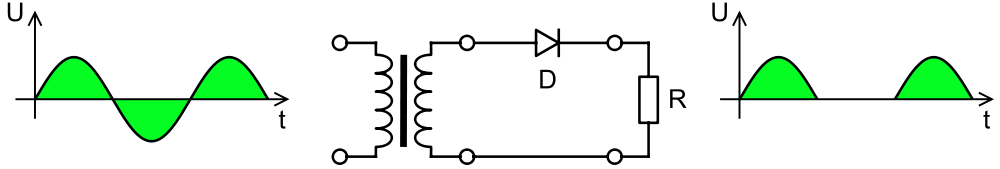
\includegraphics[width=\linewidth]{diodi_pics/1000px-Halfwave-rectifier-en-svg.png}
\end{center}

Käytännössä diodin kynnysjännite vaikuttaa tasasuunnattuun jännitteeseen. Kun muuntajalta saatavan jännitteen arvo laskee alle diodin kynnysjännitteen, tasasuuntaajan ulostulojännite on nolla volttia.

\let\thefootnote\relax\footnotetext{\tiny Kuva: \url{http://commons.wikimedia.org/wiki/File:Halfwave.rectifier.en.svg}}
 
 }

 \frame{
 \frametitle{Diodin käyttö ilmaisimena, "kidekone"}
\begin{center}
\begin{picture}(180,100)(0,0)


\vc{50,0}{}
\vl{100,0}{}
\rd{100,50}{}
\vc{150,0}{}
\vz{200,0}{}
\hln{50,0}{150}
\hln{50,50}{50}
\hln{150,50}{50}

\hgp{50,0}{}
\hln{0,50}{50}
\vln{0,50}{25}

\end{picture}
\end{center}
 }

 \frame{
 \frametitle{Kokoaaltotasasuuntaus}
\begin{center}
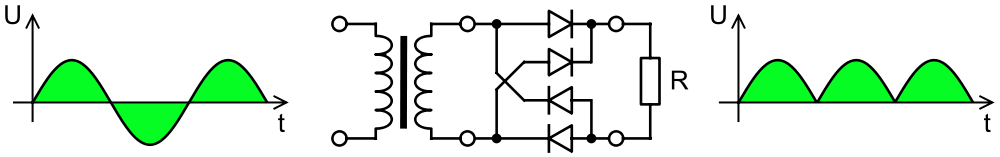
\includegraphics[width=\linewidth]{diodi_pics/1000px-Gratz-rectifier-en-svg.png}
\end{center}
\let\thefootnote\relax\footnotetext{\tiny Kuva: \url{http://commons.wikimedia.org/wiki/File:Gratz.rectifier.en.svg}}
 }

 \frame{
 \frametitle{Kokoaaltotasasuuntaus keskiulosotolla}
\begin{center}
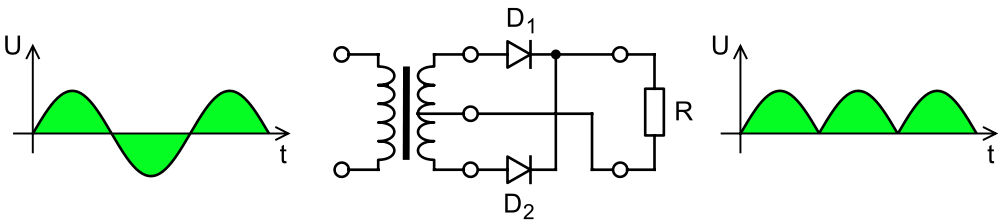
\includegraphics[width=\linewidth]{diodi_pics/1000px-Fullwave-rectifier-en-svg.png}
\end{center}
\let\thefootnote\relax\footnotetext{\tiny Kuva: \url{http://commons.wikimedia.org/wiki/File:Fullwave.rectifier.en.svg}}
 }

 \frame{
 \frametitle{Tarkkuustasasuuntaaja ja näytteenotto- ja pitopiiri}
 \begin{itemize}
 \item Operaatiovahvistimen ja diodi(e)n avulla voidaan toteuttaa myös {\em tarkkuustasasuuntaaja} sekä {\em näytteenotto- ja pitopiiri}.
 \end{itemize}
 }

 \frame{
 \frametitle{Tulon ylijännitesuojaus}
\begin{center}
\begin{picture}(200,100)(0,0)
\hln{0,0}{200}
\hln{0,50}{100}
\hln{50,100}{150}

\out{0,50}{}
\out{0,0}{}


\ud{50,50}{}
\ud{50,0}{}
\cn{50,50}

\vst{200,00}{\mbox{\tiny käyttöjännite}}

\put(100,0){\dashbox(75,75)}

\vln{200,50}{50}

\vln{137,75}{25}

\end{picture}
\end{center}



 }



 \frame{
 \frametitle{Lämpötilan mittaaminen}
 \begin{itemize}
 \item Lämpötila vaikuttaa diodin jännitteeseen, jos virta pidetään vakiona (ja päinvastoin).
 \end{itemize}
 }

 \frame{
 \frametitle{Jännitereferenssi zenerdiodilla}
\begin{center}
\begin{picture}(180,100)(0,0)
\zud{0,0}{}
\vz{0,50}{R}

\dcru{25,0}{U_{\rm Z}}

\vst{-50,25}{U}
\vln{-50,0}{25}
\vln{-50,75}{25}

\hln{-50,0}{50}
\hln{-50,100}{50}


\end{picture}
\end{center}
Jännite $U_{\rm Z}$ pysyy lähes vakiona, vaikka $U$ vaihtelee. Toiminta perustuu zenerdiodin jyrkkään ominaiskäyrään: zenerdiodin jännite ei juuri muutu, vaikka virta muuttuu.
 }


\frame{
\frametitle{Käytännön diodit}
Puolijohdediodin valintaan vaikuttavat muun muassa seuraavat ominaisuudet
\begin{itemize}
\item Virrankesto/tehonkesto
\item Jäähdytettävyys
\item Estosuuntaisen jännitteen kesto
\item Estosuuntainen kapasitanssi
\item Elpymisaika, "nopeus"
\end{itemize}
}

\frame{
\frametitle{Virrankesto, tehonkesto ja jäähdytettävyys}
\begin{itemize}
\item Liian korkea lämpötila tuhoaa komponentin.
\item Tavallinen pikkudiodi kestää suuruusluokkaa 1 W tehon.
\item Tällainen komponentti jäähtyy pääasiassa kytkentälankojen kautta.
\item Suurilla tehoilla tarvitaan jäähdytysripa ja vielä suuremmilla pakotettu ilmajäähdytys.
\item Datalehdessä yleensä arvot jatkuvalle ja hetkelliselle maksimiteholle.
\end{itemize}
}

\frame{
\frametitle{Jännitteenkesto}
\begin{itemize}
\item Liian voimakas sähkökenttä rajapinnassa aikaansaa läpilyönnin $\to$ suuri virta $\to$ komponentti palaa rikki.
\item Hallittua läpilyöntiä käytetään hyväksi zenerdiodeissa.
\end{itemize}
}

\frame{
\frametitle{Estosuuntainen kapasitanssi}
\begin{itemize}
\item Suurtaajuussovelluksissa on merkitystä rajapinnan kapasitanssilla.
\item Ilmiötä käytetään hyväksi kapasitanssidiodissa.
\end{itemize}
}


\frame{ % http://www.tokem.fi/teku/virt_amk/elko/Kurssin_sisalto/Aktiiviset/Diodit/diodit.html
\frametitle{Elpymisaika}
\begin{itemize}
\item Kun päästösuuntaan johtavassa diodissa jännite kytketään yhtäkkiä toisin päin, virta kulkee vielä hetken.
\item Schottky-diodeilla on lyhyt elpymisaika (ja matala päästösuuntainen jännite)
\end{itemize}
}

\frame{
\frametitle{Tutustu kahden  "klassikkodiodin"\ datalehtiin}
\begin{itemize}
\item Piensignaalidiodi 1N4148
\item Tasasuuntausdiodi 1N4007 
\end{itemize}
}
